\documentclass[12pt]{article}
\usepackage{setspace}
\usepackage[margin=1.0in]{geometry}
\usepackage{amsmath, amssymb, amsthm}
\usepackage{bbm}
\usepackage{graphicx}
\usepackage{float}
\usepackage{indentfirst}
\usepackage{caption}
\usepackage[labelformat=empty]{subcaption}
\usepackage{titling}
\usepackage{xcolor}
\usepackage{titling}

\newcommand{\real}{\mathbb{R}}

\setlength{\droptitle}{-1in}

%opening
\title{From Grayscale to \textcolor{red}{C}\textcolor{orange}{o}\textcolor{yellow}{l}\textcolor{green}{o}\textcolor{blue}{r}\textcolor{purple}{:}\\Digital Image Colorization using Machine Learning}
\author{Cris Zanoci and Jim Andress}
\date{November 15, 2015}

\begin{document}

\maketitle

\section{Introduction}
\label{sec:intro}


\section{Methods}
\label{sec:methods}

Our colorization algorithm is as follows.  We begin by discretizing the colors of the training image using k-means clustering.  Rather than running the k-means over the three dimensional $RGB$ coordinates of each pixel, we instead convert the input images to the $L\alpha\beta$ color space, where $L$ represents the luminance of a pixel and $\alpha, \beta$ are the two components of its color.  This space is specifically designed to match a human's perception of color, which means that the centroids produced through clustering will represent a natural division of the colors. For k-means, we typically use 32 colors. By running our algorithm with various values of $k$, we have found that using more than 32 colors does not improve the results. 

Next, we extract a feature vector at every pixel of the training image and use PCA to reduce its dimension as described in Section \ref{sec:dataset}. Then we train a set of SVMs, one per discretized color. We use a one vs. all classification procedure, which means that each SVM predicts whether or not a pixel has its corresponding color. To be less sensitive to outlier pixels, we employ $\ell_1$ regularization:
\begin{align}
    \label{eq:SVM}
    \min_{b, w} \dfrac{1}{2} \|w\|^2 &+ C \sum_{i} \xi_i \\
    \text{s.t. } y^{(i)}(w^Tx^{(i)}+b) &\geq 1-\xi_i, i = 1, 2, ..., m \\
    \xi_i &\geq 0, i = 1, 2, ..., m
\end{align}
where $C$ is a parameter that we can vary. We tried using two types of kernels, RBF and linear, and chose the latter as it yields comparable results while also being significantly faster.

For testing, we read in the grayscale image, compute the feature vector at every pixel and project it into the subspace determined by PCA in the training step. At this point, it is tempting to simply run the SVMs on each pixel and assign the color of the maximum-margin SVM.  However, this would completely disregard the spatial coherency element of image colorization.  Instead, we make the reasonable assumption that colors are most likely to change where there are edges in the luminance channel of the image.  We therefore use the Sobel operator to approximate the norm of the gradient of the luminance at each pixel. If we treat the image as a graph with edges connecting pixels, then values computed by the Sobel operator indicate how weakly a pixel couples to its neighbors. 
After computing the SVM margins and Sobel edge weights at each pixel in the training image, we feed all of this information into the energy minimization problem with cost function
\begin{equation}
    \label{eq:energy_min}
    \alpha \sum_p -s_{c(p)} (p) + \sum_{p,q \in \mathcal{N}(p)} \frac{\| c(p) - c(q) \|} {2(w(p)^{-1} + w(q)^{-1})^{-1}}
\end{equation}
Here $p$ is a pixel, $\mathcal{N}(\cdot)$ represents a pixel's eight neighbors, $c(\cdot)$ is the color chosen for a particular pixel, $s_{c} (\cdot)$ is the margin when the SVM associated with color $c$ is used to classify a pixel, and $w(\cdot)$ is the Sobel edge weight at a pixel.

Although it seems like finding the color assignment which minimizes Equation $\ref{eq:energy_min}$ would be difficult (in many cases this problem is, in fact, NP-hard), we can use the Boykov-Kolmogorov algorithm to efficiently compute approximate solutions \cite{boykov2001fast, boykov2004experimental}.  This algorithm works by iteratively expanding the set of pixels given a particular color by constructing a graph in which each pixel is connected to its neighbors, a node $n_1$ representing the color being expanded, and a node $n_2$ representing all other colors, each with appropriate weights.  By computing a minimum cut of this graph, we are left with some pixel nodes connected to $n_1$ and some to $n_2$, but none connected to both.  We then expand the labelling so that the nodes connected to $n_1$ are given the color associated with it and the others remain the same.  This procedure is proven to converge to within a known factor of the global optimum, and typically finishes in tens of seconds for images with $600 \times 400$ pixels.

\section{Results}
\label{sec:results}

The results of our baseline implementation are presented in Fig. \ref{fig:baseline_result}. Even though we managed to transfer the color to most of the vegetation and the sky, the upper right corner of the sky and some parts of the mountain are miscolored. This defect and the long overall execution time motivated us to search for other methods. 

For the second approach, we use $7\times7$ square to extract information about the neighborhood of each pixel. This results in a 49-dimensional feature space, which later gets reduced using PCA to 20, and then 10 dimensions. We use a grid that samples roughly $4\%$ of the colored picture. 

Figure \ref{fig:elephants} shows the application of the algorithm described in section \ref{sec:dct}. Note that even though many of the points inside the elephant's body were attributed the wrong label (c), our voting procedure relabels those points to achieve a consistent texture (d). Figure (e) shows that we are most confident in the labels attributed to the sky. This makes perfect sense, since the majority of the training image was the blue sky and hence it will make up most of the colorized image. Figure \ref{fig:algo_compare} demonstrates the improvement of our second approach over the naive baseline. 

\section{Future Work}
\label{sec:next}

Since the above method clearly has its shortcomings, we will investigate more novel techniques, like Parzen windows, structured-SVMs, Markov Random Fields and maybe neural networks.

\pagebreak
\section{Appendix}
\begin{figure}[H]
    \centering
    \begin{subfigure}{2.1in}
        \centering
        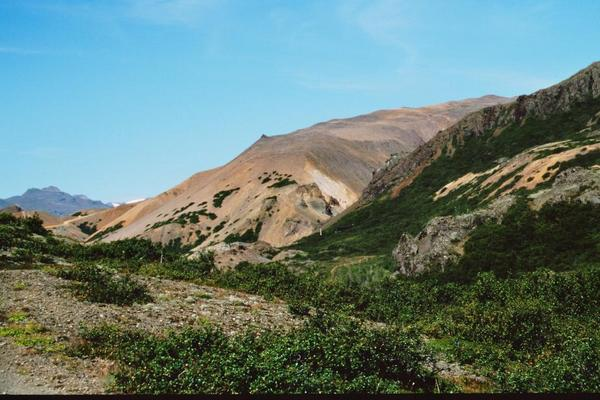
\includegraphics[width=2in]{./Images/mountain_color.jpg}
        \caption{(\textbf{a})}
    \end{subfigure}
    \begin{subfigure}{2.1in}
        \centering
        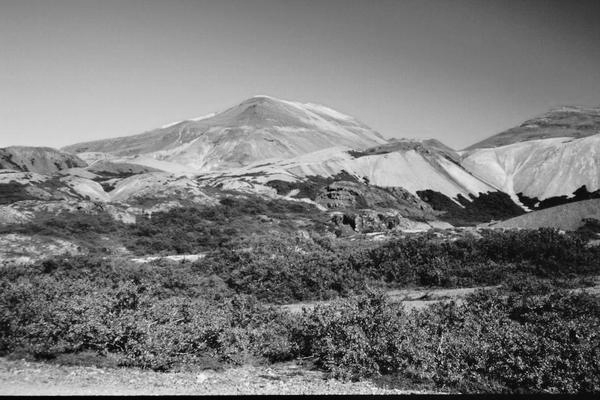
\includegraphics[width=2in]{./Images/mountain_gray.png}
        \caption{(\textbf{b})}
    \end{subfigure}
    \begin{subfigure}{2.1in}
        \centering
        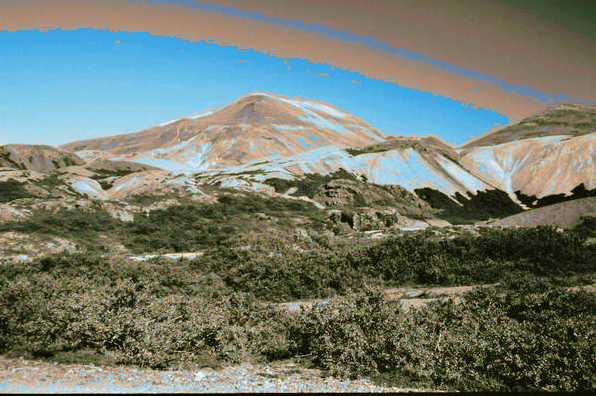
\includegraphics[width=2in]{./Images/mountain_gray_colored_40.png}
        \caption{(\textbf{c})}
    \end{subfigure}
    \caption{The baseline colorization procedure. (\textbf{a}) A colored training image. (\textbf{b}) A gray-scale test image. (\textbf{c})  A colorized version of the test image.}
    \label{fig:baseline_result}
\end{figure}

\begin{figure}[H]
    \centering
    \begin{subfigure}{2.1in}
        \centering
        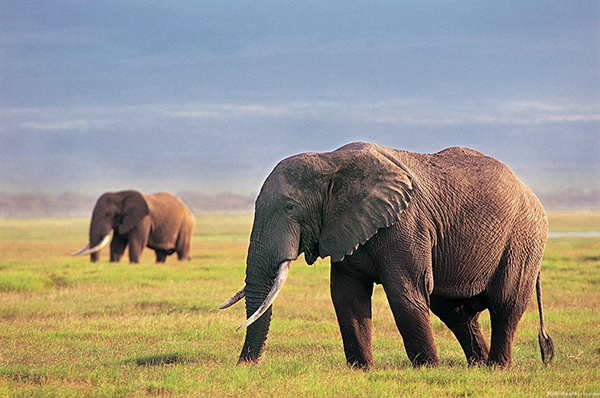
\includegraphics[width=2in]{./Images/elephant2.jpg}
        \caption{(\textbf{a})}
    \end{subfigure}
    \begin{subfigure}{2.1in}
        \centering
        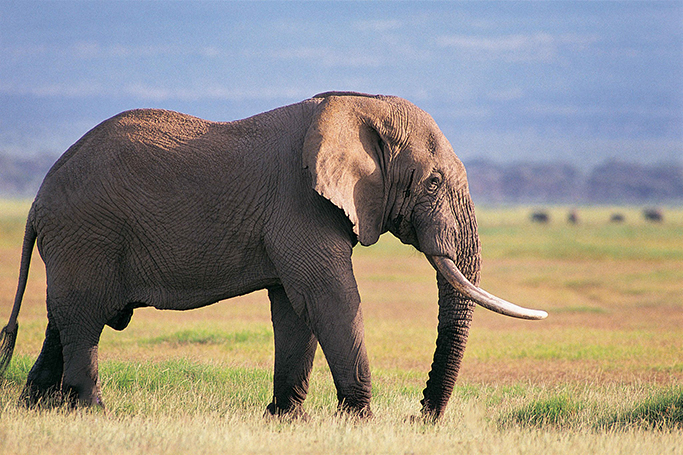
\includegraphics[width=2in]{./Images/elephant1.jpg}
        \caption{(\textbf{b})}
    \end{subfigure}
    \begin{subfigure}{2.1in}
        \centering
        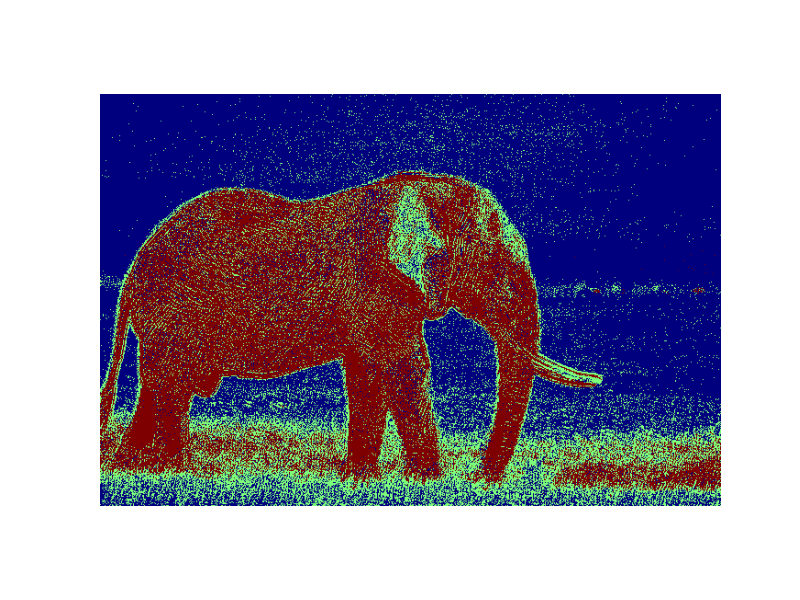
\includegraphics[width=2in]{./Images/2.png}
        \caption{(\textbf{c})}
    \end{subfigure}
    \newline
    \begin{subfigure}{2.1in}
        \centering
        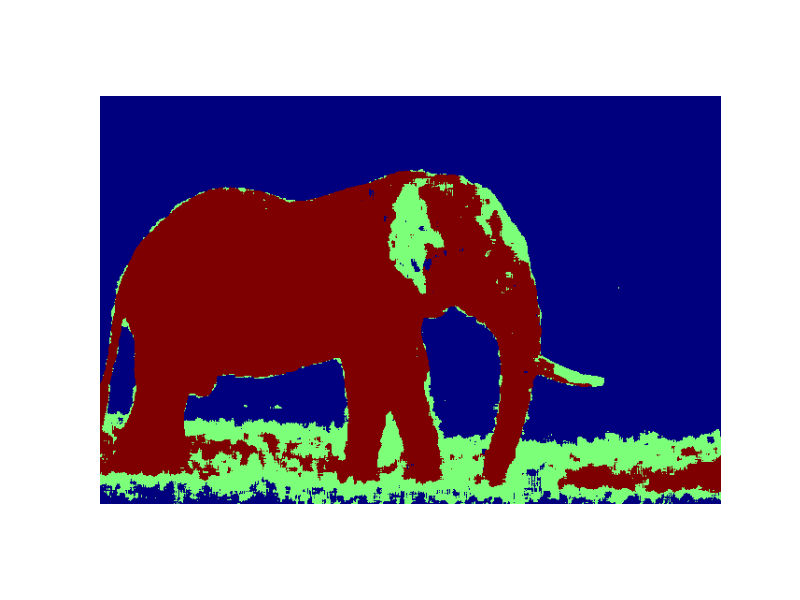
\includegraphics[width=2in]{./Images/3.png}
        \caption{(\textbf{d})}
    \end{subfigure}
    \begin{subfigure}{2.1in}
        \centering
        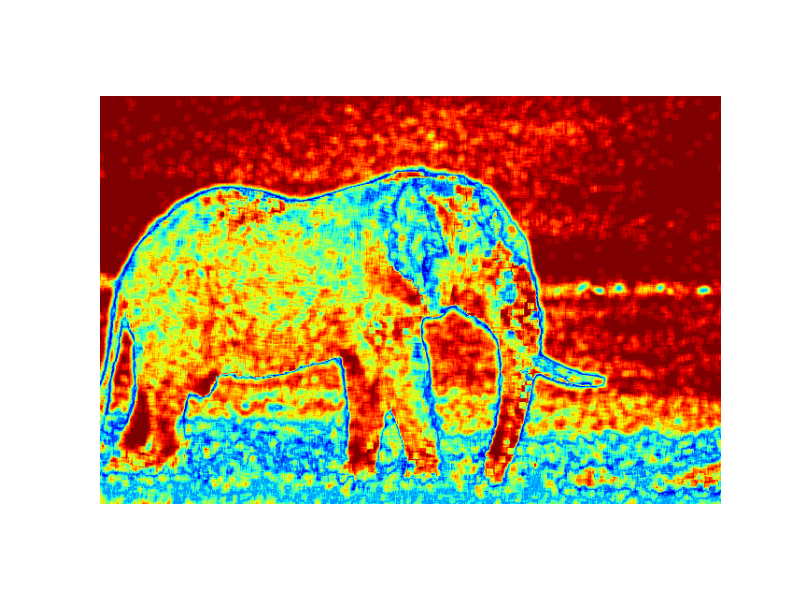
\includegraphics[width=2in]{./Images/4.png}
        \caption{(\textbf{e})}
    \end{subfigure}
    \begin{subfigure}{2.1in}
        \centering
        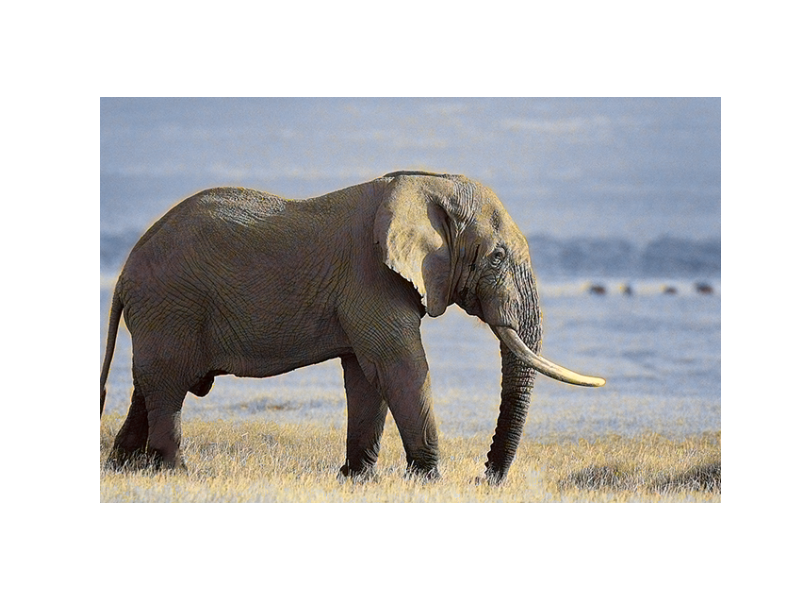
\includegraphics[width=2in]{./Images/5.png}
        \caption{(\textbf{f})}
    \end{subfigure}
    \caption{The more complicated colorization procedure. (\textbf{a}) A colored training image. (\textbf{b}) The test image with the orginal color. (\textbf{c})  The results of running kNN on the test image. (\textbf{d})  The results of image-space voting on the kNN results. (\textbf{e})  The confidence of each pixel's prediction. (\textbf{f})  The colorized version of the test image.}
    \label{fig:elephants}
\end{figure}

\begin{figure}[H]
    \centering
    \begin{subfigure}{3.1in}
        \centering
        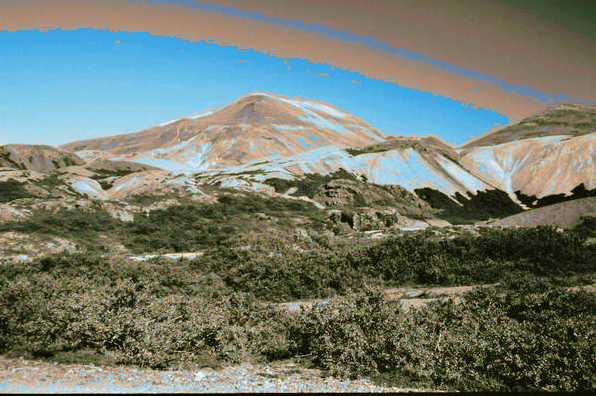
\includegraphics[width=3in]{./Images/mountain_gray_colored_40.png}
        \caption{(\textbf{a})}
    \end{subfigure}
    \begin{subfigure}{3.1in}
        \centering
        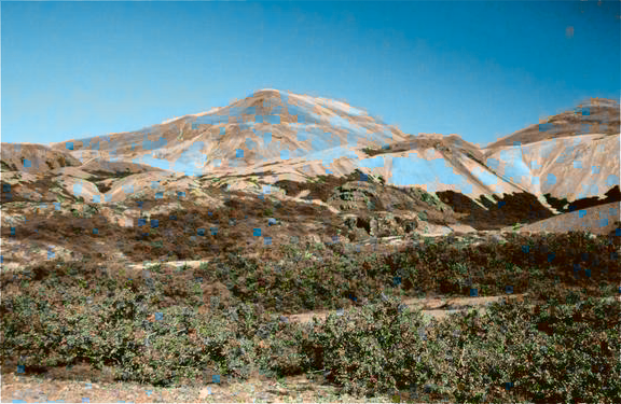
\includegraphics[width=3in]{./Images/landscape_5.png}
        \caption{(\textbf{b})}
    \end{subfigure}
    \caption{A comparison of our baseline and more complicated colorization results. (\textbf{a}) The baseline colorization. (\textbf{b}) Our more complex colorization.}
    \label{fig:algo_compare}
\end{figure}

\newpage

\bibliographystyle{ieeetr}
\bibliography{references}

\end{document}
